\documentclass[11pt]{article}
\renewcommand{\baselinestretch}{1.05}
\usepackage{amsmath,amsthm,verbatim,amssymb,amsfonts,amscd,graphicx,enumitem}
\usepackage{tikz,pgfplots,multicol}

\usepackage{graphics}
\topmargin0.0cm
\headheight0.0cm
\headsep0.0cm
\oddsidemargin0.0cm
\textheight23.0cm
\textwidth16.5cm
\footskip1.0cm
\theoremstyle{plain}
\newtheorem{theorem}{Theorem}
\newtheorem{corollary}{Corollary}
\newtheorem{lemma}{Lemma}
\newtheorem{proposition}{Proposition}
\newtheorem*{surfacecor}{Corollary 1}
\newtheorem{conjecture}{Conjecture} 
\newtheorem{question}{Question} 
\theoremstyle{definition}
\newtheorem{definition}{Definition}
\graphicspath{ {images/} }


\newcommand*{\boxedcolor}{purple}
\makeatletter
\renewcommand{\boxed}[1]{\textcolor{\boxedcolor}{%
  \fbox{\normalcolor\m@th$\displaystyle#1$}}}
\makeatother

\begin{document}
 


\title{Calculus 1, Spring 2017}
\author{John Keller}
\maketitle



\subsection{A Preview of Calculus}

\subsection{The Area Problem}

\includegraphics[width=\textwidth]{01-fig2.pdf}

Let $A_n$ be the area of the inscribed polygons with $n$ sides. As $n$ increases, it appears that $A_n$ becomes closer and closer to the area of the circle. We say that the area of the circle is the limit of the areas of the inscribed polygons, and we write: $$A=\lim_{n\to\infty} A_n$$

\subsection{The Tangent Problem}

\subsection{Velocity}

Let's examine the motion of a car that travels along a straight road and assume that we can measure the distance by the car (in feet) at 1-second intervals as in the following chart:

\begin{table}[h!]
\centering
 \begin{tabular}{|c|c|c|c|c|c|c|} 
 \hline
 $t=$ Time elapsed (s) & 0 & 1 & 2 & 3 & 4 & 5 \\
 \hline
 $d=$ Distance (ft) & 0 & 2 & 9 & 24 & 42 & 71 \\
 \hline
 \end{tabular}
\end{table}


$$\text{average velocity}=\frac{\text{change in position}}{\text{time elapsed}}$$


\subsection{The Limit of a Sequence}

	The notation $$\lim_{n\to\infty} a_n = L$$ is used if the terms $a_n$ approach the number $L$ as $n$ becomes large. This means that the numbers $a_n$ can be made as close as we like to the number $L$ by taking $n$ sufficiently large.


\section{Functions and Models}

\subsection{Four Ways to Represent a Function}

\begin{description}[style=nextline]
	\item[Function] A graph with only one $x$ and $y$ value pair
   	\item[Domain] All possible $x$ values of the function.
  	\item[Range] All possible $y$ values of the function.
  	\item[Independent variable] A symbol that represents an arbitrary number in the domain of $f$.
  	\item[Dependent variable] A symbol that represents a number in the range of $f$.
  	\item[Even function] A function which has symmetry across the y-axis. In addition, $f$ must satisfy $f(-x)=f(x)$.
  	\item[Odd function] A function that has symmetry along both the x and y-axis. In addition, $f$ must satisfy $f(-x)=-f(x)$.
\end{description}

\begin{figure}[h]
	\includegraphics[width=200px]{images/Even_vs_Odd_Parity}	
\end{figure}

\paragraph{Representations of Functions} 
	There are many ways to represent the actions of a function; sometimes it is helpful to think of a function as a machine.
	
	\begin{figure}[h]
		\includegraphics{images/11-fig2}	
	\end{figure}

\paragraph{Sample Problems}
\begin{enumerate}
  \item Determine whether each of the following functions is even, odd, or neither even nor odd.
  \begin{enumerate}
     \item $f(x)=x^5+x$
     \item $g(x)=1-x^4$
     \item $h(x)=2x-x^2$
   \end{enumerate}
  \item The numbers starts at 1 with every call to the enumerate environment.
\end{enumerate}

\subsection{Mathematical Models: A Catalog of Essential Functions}
\begin{description}[style=nextline]
	\item[Mathematical model] A mathematical description (often by means of a function or an equation) of a real-world phenomenon such as the size of a population, the demand for a product, the speed of a falling object.
\end{description}
\begin{figure}[h]
	\includegraphics{images/12-fig1}	
\end{figure}
\begin{description}[style=nextline]
	\item[Linear function] The graph of a function is a straight line, taking the form of $y=mx+b$ where $m$ is the slope of the line and $b$ is the y-intercept.
	\item[Empirical model] When there is no physical law or principle to help us formulate a model, based entirely on collected data.
	\item[Linear regression model] A linear line of best fit for a given set of data
\end{description}

\subsection{New Functions from Old Functions}

\subsubsection{Vertical and Horizontal Shifts (assuming $c>0$)}

\begin{itemize}
	\item $y=f(x)+c$ shifts the graph $c$ units \textbf{up}
	\item $y=f(x)-c$ shifts the graph $c$ units \textbf{down}
	\item $y=f(x-c)$ shifts the graph $c$ units to the \textbf{right}
	\item $y=f(x+c)$ shifts the graph $c$ units to the \textbf{left}	
\end{itemize}

\subsubsection{Vertical and Horizontal Stretching and Reflecting (assuming $c>1$)}

\begin{itemize}
	\item $y=cf(x)$ \textbf{stretches} the graph $y=f(x)$ \textbf{vertically} by a factor of $c$.
	\item $y=(\frac{1}{c})f(x)$ \textbf{shrinks} the graph of $y=f(x)$ \textbf{vertically} by a factor of $c$.
	\item $y=f(cx)$ \textbf{shrinks} the graph of $y=f(x)$ \textbf{horizontally} by a factor of $c$.
	\item $y=f(\frac{x}{c})$ \textbf{stretches} the graph of $y=f(x)$ \textbf{horizontally} by a factor of $c$.
	\item $y=-f(x)$ \textbf{reflects} the graph of $y=f(x)$ about the $x$-axis.
	\item $y=f(-x)$ \textbf{reflects} the graph of $y=f(x)$ about the $y$-axis.
\end{itemize}



\subsection{Graphing Calculators and Computers}

Nope

\subsection{Exponential Functions}




\subsection{Inverse Functions and Logarithms}

\begin{description}[style=nextline]
	\item[One-to-one Function] It never takes the same value twice
	\item[Horizontal Line Test] A method for testing if a function is one-to-one. 	
	\item[Inverse Function] Switching $x$ and $y$ in the equation and then reformatting into a $y=$ form.
\end{description}

\subsubsection{Laws of Logarithms}
\begin{itemize}
	\item $\log_a(xy)=\log_a x + \log_a y$
	\item $\log_a(\frac{x}{y})=\log_a x - \log_a y$
	\item $\log_a(x^r)=r \log_a x$ (where $r$ is any real number)
\end{itemize}

\subsubsection{Natural Logarithms}
\begin{itemize}
	\item $\log_e x = \ln x$
	\item $\ln e = 1$
\end{itemize}




\subsection{Parametric Curves}

\section{Bleh}

\subsection{Tangent & Velocity}

\subsubsection{The Velocity Problem}

Example: Suppose a rock is dropped off a cliff that's hight is given by: $$h(t)=-16t^2\ \textbf{(ft)}$$

Question: What is the instantaneous velocity of the rock at $t=3$ seconds.

All we can do is compute the average velocities over shorter and shorter time intervals.

$$\text{Average velocity} = \frac{\text{change in position}}{\text{time elapsed}} = \frac{h(t_2)-h(t_1)}{t_2-t_1}$$

\subsubsection{The Tangent Problem}




\subsection{The Limit of a Function}
 
 
$$\underset{x \rightarrow a}{\text{lim}}f(x)=L$$ can be written as "the limit of $f(x)$ as $x$ approaches $a$ = $L$"


\begin{minipage}[t]{.3\textwidth}

\begin{figure}
\pgfplotsset{compat=1.6,width=5cm,height=5cm}
\pgfplotsset{soldot/.style={color=blue,only marks,mark=*}} \pgfplotsset{holdot/.style={color=blue,fill=white,only marks,mark=*}}
		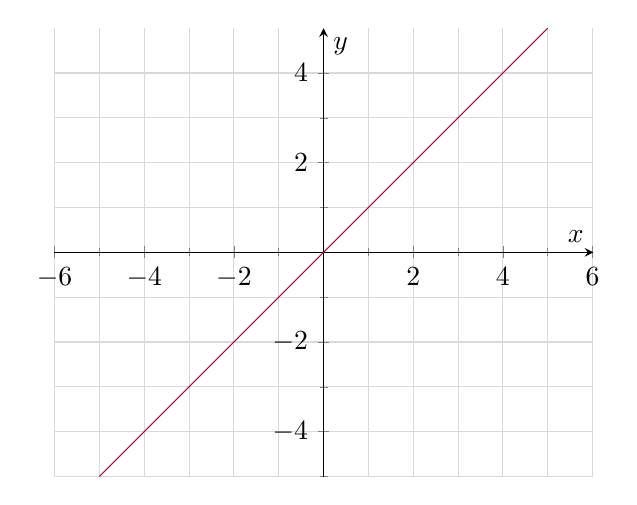
\begin{tikzpicture}
		\begin{axis}[axis lines=middle,xlabel=$x$,ylabel=$y$,axis equal,grid=both,minor tick num=1,grid style={solid, gray!30}]
			\addplot[purple] {x};
		\end{axis}
	\end{tikzpicture}
\caption{$f(x)=x$}
\end{figure}

\end{minipage}% 
\begin{minipage}[t]{.3\textwidth}
This is \\
some different \\
text, right-aligned \\
for demo purposes, \\
and with more lines.
\end{minipage}%
\begin{minipage}[t]{.3\textwidth}
This is \\
some different \\
text, right-aligned \\
for demo purposes, \\
and with more lines.
\end{minipage}

 \subsection{___}
 
\subsection{Continuity}
\subsubsection{Def:} A function is \textbf{continuous} at the number $a$ if $$\underset{x \rightarrow a}{\text{lim}}f(x)=f(a)$$. In other words, $f$ is continuous at $a$ id $f$ satisfies the direct substitution property at $a$.


Actually says these three things:
\begin{enumerate}
	\item $f(a)$ is defined ($a$ is in the domain of $f(x)$)
	\item $\underset{x\rightarrow a^-}{\text{lim}}=\underset{x \rightarrow a^+}{\text{lim}} f(x)$, $\Big[\underset{x \rightarrow a}{\text{lim}}\text{ exists}\Big]$
	\item $\underset{x\rightarrow a}{\text{lim}}f(x)=f(a)$
\end{enumerate}
Which can be thought of as a checklist
\begin{itemize}
	\item Our main focus today (and on midterm 1) is piecewise functions.
	\item In general, we can think of the entire function as continuous \textbf{except} where the function jumps.
	\item This is because of the theorem below
\end{itemize}

\subsubsection{Theorem:} The following functions are continuous everywhere on their domains:
\begin{enumerate}
	\item Polynomials
	\item Rational Functions
	\item Root Functions
	\item Exponentials
	\item Logs
	\item Trig
\end{enumerate}

\textbf{Exercise}: What are the domains in each case?
 
 
 
 \subsubsection{Example 1}
 $$f(x)=\frac{x^2-x}{x^2-1} \qquad a=1$$
 
Let's check out criteria and see what happens:
 \begin{enumerate}
 	\item $f(1)$ is defined
 	\item $\underset{x \rightarrow 1}{\text{lim}}f(x) = \underset{x \rightarrow 1}{\text{lim}} \frac{x^2-x}{x^2-1} = \frac{1}{1+1}=\frac{1}{2}$
 	\item $\underset{x \rightarrow 1}{\text{lim}}f(x)\neq f(1)$
 \end{enumerate}

This means: $f$ is not defined at -1 so $f$ is not continuous at -1.

The biggest problem is descerning between number 2 and number 3


\subsubsection{Example 2}
\begin{itemize}
	\item Another type of problem involves choosing the correct constant in order to make a piecewise function continuous on $(-\infty, \infty)$
\end{itemize}

For what constant $c$ is the following function continuous on $(-\infty, \infty)$.

$$f(x)=\begin{cases} 
      		cx+1 & x < 1 \\
      		x^2-c & x \geq 1 
   		\end{cases}$$

\begin{itemize}
	\item Since this is piecewise and both pieces are polynomials, we need to only focus on continuity at $a=1$.
	\item Let's check our criteria:
\end{itemize}

\begin{enumerate}
	\item $f(1)$ is defined, $f(1)=1-c$.
	\item LHL: $\underset{x\rightarrow 1^-}{\text{lim}}= \underset{x\rightarrow 1^-}{\text{lim}}(x+2)=x+2$ \\
		RHL: $\underset{x\rightarrow 1^+}{\text{lim}}= \underset{x\rightarrow 1^+}{\text{lim}}(x^2-c)=1-c$
	\item If you've done part 2 correctly, you don't even need to check this. So $c=\frac{1}{2}$ makes $f$ continous on $(-\infty,\infty)$
\end{enumerate}

\textbf{Caution:} You must argue using limits! It's not enough to just plug in $a$ to each piece and solve for $c$.


\subsubsection{Intermediate Value Theorem (IVT)}

\begin{center}\includegraphics[width=5cm]{images/IntermediateValueTheoremGraph}\end{center}

\begin{itemize}
	\item Suppose $f$ is continuous on the closed interval $[a,b]$, and that $N$ is a number between $f(a)$ and $f(b)$, where $f(a)\neq f(b)$. 
	\item Then there exists a number $C$ in the open interval $(a,b)$ such that $f(c)=N$
	\item In other words, $f$ assumes every value between $f(a)$ and $f(b)$, possibly more than once.
	\item Primarily used to find roots of equations in a given interval
	\item \textbf{Note:} To use the IVT, you must produce a continuous function on a closed interval.
\end{itemize}


\section{Differentiation Rules}

\subsection{Derivatives of Polynomials and Exponential Functions}

\begin{enumerate}
	\item \textbf{Power Rule}\textit{ (the most basic one)}:$$\begin{align}
		f(x)&=x^n\\
		f'(x)&=nx^{n-1}
	\end{align}$$
	\item \textbf{Product Rule:}$$\begin{align}
		f(x)&=g(x)\cdot h(x)\\
		f'(x)&= g'(x)\cdot h(x) + g(x) \cdot h'(x)
	\end{align}$$
	\item \textbf{Quotient Rule:}$$\begin{align}
		f(x)&=\frac{g(x)}{h(x)}\\
		f'(x)&= \frac{g'(x)\cdot h(x) - g(x) \cdot h'(x)}{[h(x)]^2}
	\end{align}$$
	\item \textbf{Chain Rule} \textit{(used for nested functions)}: $$\begin{align}
		f(x)&=g(h(x))\\
		f'(x)&=g'(h(x))\cdot h'(x)
	\end{align}$$
	\item \textbf{Sum \& Difference Rules:}\\ \\
	\begin{minipage}{.5\linewidth}
		$$\begin{align}
		f(x)&=g(x)+h(x)\\
		f'(x)&=g'(x)+h'(x)
		\end{align}$$
	\end{minipage}
	\begin{minipage}{.5\linewidth}
	$$\begin{align}
		f(x)&=g(x)-h(x)\\
		f'(x)&=g'(x)-h'(x)
	\end{align}$$
	\end{minipage}

	\item \textbf{Constant Rules:}\\ \\
	\begin{minipage}{.3\linewidth}
		$$\begin{align}
		f(x)&=c\\
		f'(x)&=0
		\end{align}$$
	\end{minipage}
	\begin{minipage}{.3\linewidth}
	$$\begin{align}
		f(x)&=c\cdot g(x)\\
		f'(x)&=c\cdot g'(x)
	\end{align}$$
	\end{minipage}
	\begin{minipage}{.3\linewidth}
	$$\begin{align}
		f(x)&=c x\\
		f'(x)&= c
	\end{align}$$
	\end{minipage}
\end{enumerate}

\textbf{Definition of the Number $e$}
$$e \text{ is the number such that  }\underset{h\rightarrow 0}{\text{lim}}\frac{e^h-1}{h}=1$$

\textbf{Derivative of the Natural Exponential Function}
$$\frac{d}{dx}(e^x)=e^x$$

\subsection{3.2}

\subsection{Derivatives of Trigonometric Functions}

\begin{enumerate}
	\item $$\underset{h\rightarrow 0}{\text{lim}}\sin x \cdot \underset{h\rightarrow 0}{\text{lim}}\frac{\cos h -1}{h}+\underset{h\rightarrow 0}{\text{lim}}\cos x \cdot \underset{h\rightarrow 0}{\text{lim}}\frac{\sin h}{h}$$
	\item $$\underset{\theta \rightarrow 0}{\text{lim}}\frac{\sin\theta}{\theta}=1$$
	\item $$\underset{\theta \rightarrow 0}{\text{lim}}\frac{\cos\theta-1}{\theta}=0$$
	\item $$\frac{d}{dx}(\sin x)=\cos x$$
	\item $$\frac{d}{dx}(\cos x)=-\sin x$$
	\item $$\frac{d}{dx}(\tan x)=\text{sec}^2 x$$
\end{enumerate}

\subsection{The Chain Rule}

\begin{enumerate}
	\item \textbf{The Chain Rule} If $g$ is differentiable at $x$ and $f$ is differentiable at $g(x)$, then the composite function $F=f\circ g$ defined by $F(x)=f(g(x))$ is differentiable at $x$ and $F'$ is given by the product $$\boxed{F'(x)=f'(g(x)) \cdot g'(x)}$$ In Leibniz notation, if $y=f(u)$ and $u=g(x)$ are both differentiable functions, then $$\frac{dy}{dx}=\frac{dy}{du}\frac{du}{dx}$$
	\item \textbf{The Power Rule Combined with the Chain Rule} If $n$ is any real number and $u=g(x)$ is differentiable, then $$\boxed{\frac{d}{dx}(u^n)=nu^{n-1}\frac{du}{dx}}$$ Alternatively, $$\frac{d}{dx}[g(x)]^n=n[g(x)]^{n-1}\cdot g'(x)$$
	\item \textbf{Derivative of $\boldsymbol{a^x}$ for general base $\boldsymbol{a}$} $$\boxed{\frac{d}{dx}(a^x)=a^x\ln a}$$
\end{enumerate}


\section{4}
\subsection{Related Rates}
\textbf{How to Solve related rates}
\begin{enumerate}
	\item Draw a picutre
	\item Assign variables to whatever quantities are in your picture
	\item Write what is given and what is unknown in terms of these variables
	\item Relate variables by an equation (usually involves geometry)
	\item Take $\frac{d}{dt}$ of both sides of the relation from 4 and implicitly differentiate
	\item Plug in known quantities, solve for unknown
\end{enumerate}
\end{document}